\begin{figure}[!tp]
    \centering
    \setlength{\abovecaptionskip}{4pt}
    \setlength{\belowcaptionskip}{-8pt}
    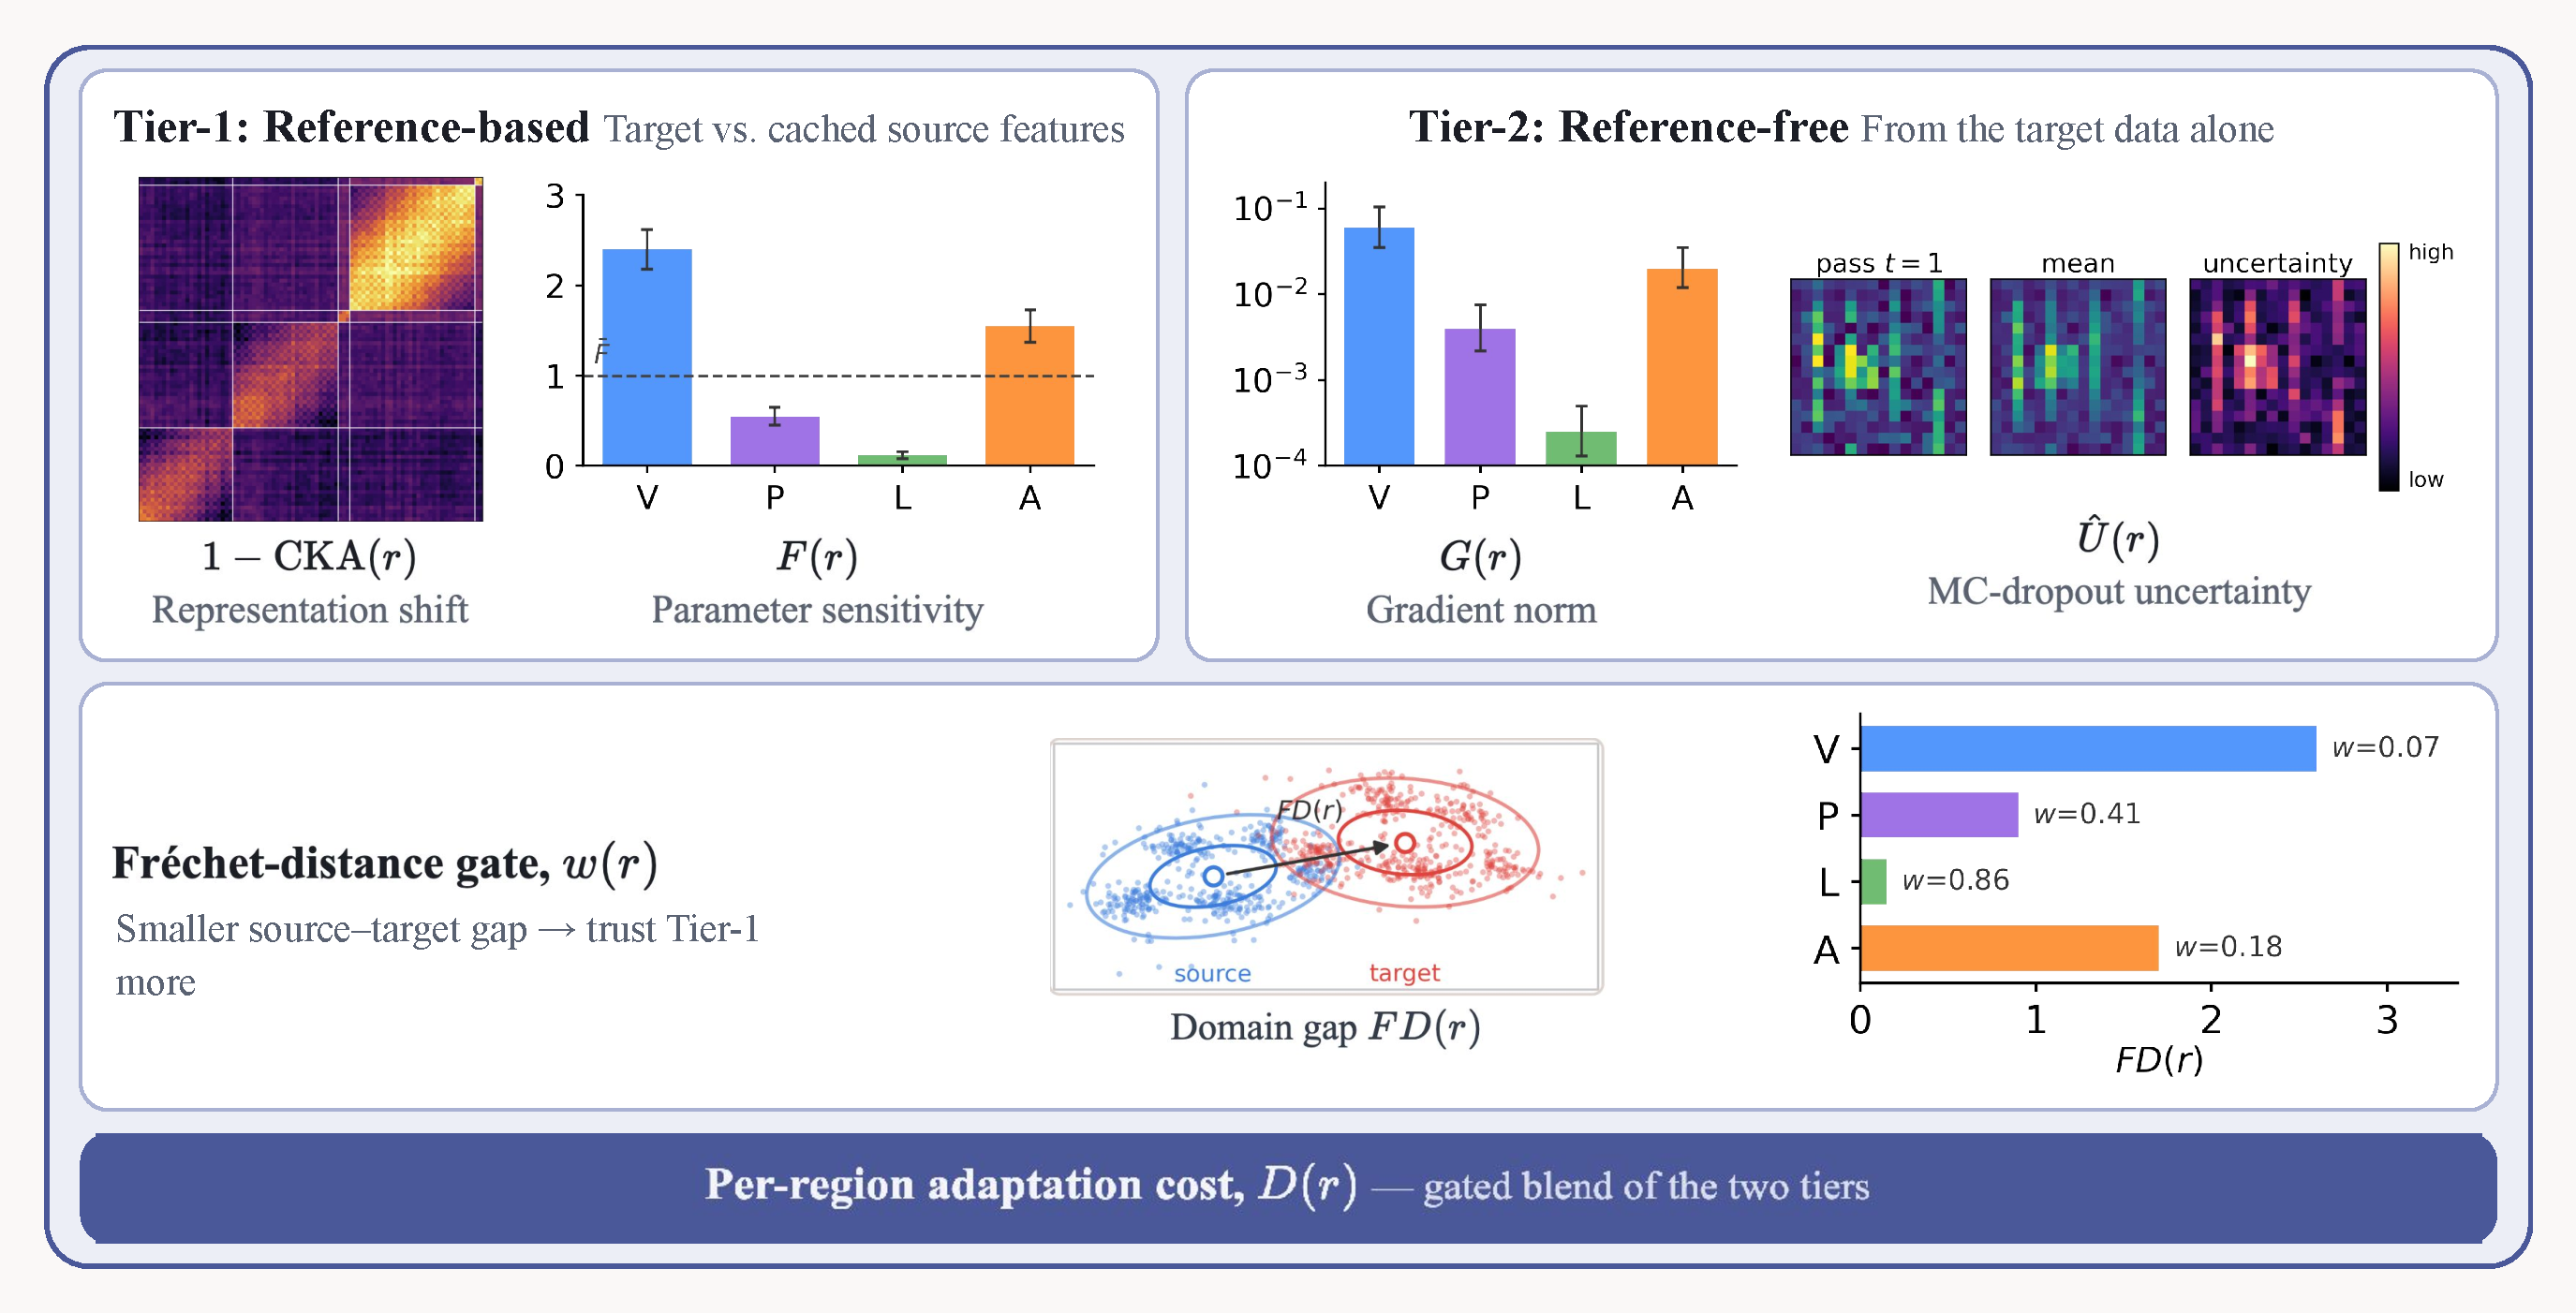
\includegraphics[width=\columnwidth]{images/diagnostic_figure.pdf}
    \caption{\textbf{The two-tier diagnostic.} Tier~1 scores representational shift ($1 - \mathrm{CKA}(r)$) against the cached source reference, weighted by Fisher sensitivity $\overline{F}(r)$ normalized to a global mean of one (dashed line); Tier~2 profiles the surrogate gradient norm $G(r)$ and MC Dropout uncertainty $\hat{U}(r)$ from target observations alone; the gate $w(r) = \exp(-\gamma \cdot \mathrm{FD}(r))$ trusts Tier~1 where the source--target gap is small, and the blend yields $D(r)$. V, P, L, and A denote vision encoder, projector, language backbone, and action head.}
    \label{fig:diagnostic}
\end{figure}